\shorthandoff{"}
\chapter{Forschungsergebnisse}
\label{ch:ergebnisse}

\section{Fähigkeiten und Präferenzen der Mitarbeiter}
\label{ch:ergebnisse:analyse}
An der Umfrage unter den Projektmitarbeitern haben N=23 Personen aus dem Fachbereich \acl{JES} der EXXETA AG teilgenommen. Diese Angestellten haben insgesamt 643 Kompetenzbewertungen im Intranet des Unternehmens abgegeben. Dies entspricht ca. 28 vergebenen Beurteilungen pro Person. Die Bewertungen verteilen sich auf 212 der \anzFaehigkeiten unterschiedlichen, im Intranet gespeicherten Fähigkeiten. Java ist mit 16 Beurteilungen die meist beherrschte Kompetenz.

Bei der Umfrage zu den Präferenzen haben die Mitarbeiter insgesamt 1408 Bewertungen abgegeben, welche sich auf 370 einzelne Kompetenzen verteilen. Dies entspricht knapp über 61 abgegebenen Wünschen pro Mitarbeiter. Git ist mit 18 Beurteilungen die meist präferierte Fähigkeit.

Abbildung \ref{fig:ergebnisse:analyse:abb1}, dass sowohl bei Darstellung der beherrschten Fähigkeiten als auch der präferierten Kompetenzen der in Kapitel \ref{ch:empfehlungssysteme:cf:speicherbasiert} vorgestellte lange (Ratten-)Schwanz gut erkennbar ist. Dieser ist in beiden Fällen jedoch weniger stark ausgeprägt, als in der Referenzdarstellung aus Abbildung \ref{fig:empfehlungssysteme:cf:speicherbasiert:abb1}.

\begin{figure}[h]
	\centering
	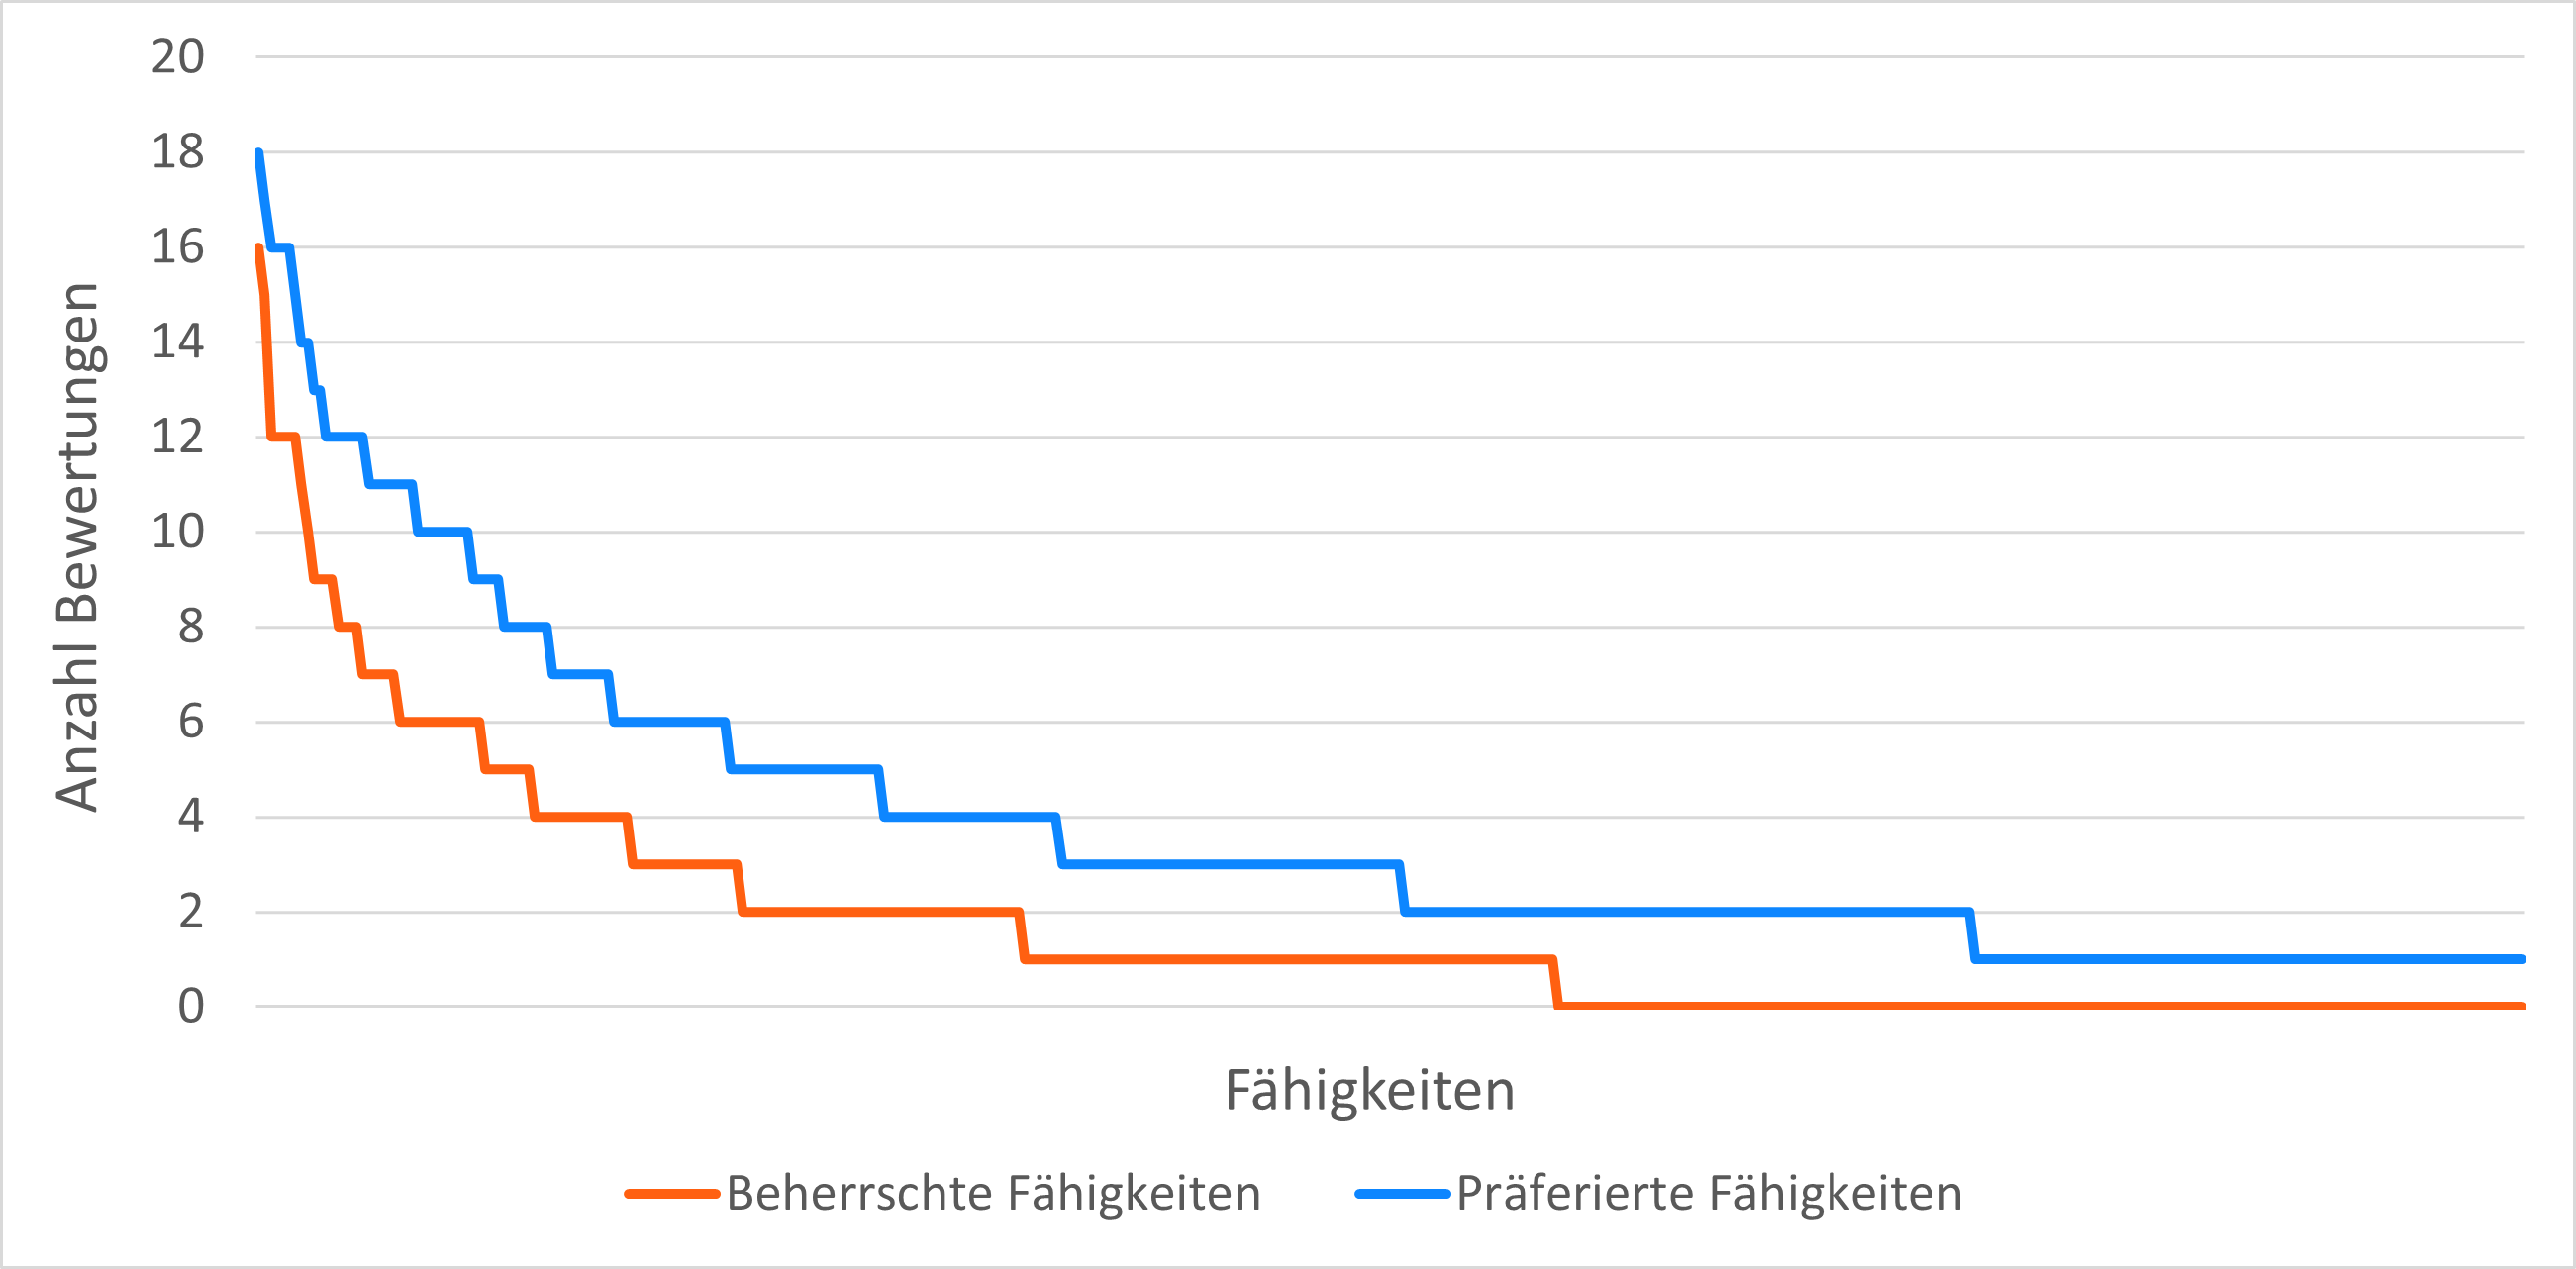
\includegraphics[width=1\textwidth]{gfx/long-tail-insgesamt.png}
	\caption{Langer (Ratten-)Schwanz bei den Fähigkeitsbewertungen im EXXETA-Intranet}
	\label{fig:ergebnisse:analyse:abb1}
\end{figure}

Bei der gemeinsamen Betrachtung von Kompetenzen und Wünschen ist auf Mitarbeiterebene festzustellen, dass ein durchschnittlicher Angestellter etwa 74.7 Fähigkeiten beherrscht und/oder präferiert. Abbildung \ref{fig:ergebnisse:analyse:abb3} zeigt, wie viele dieser Kompetenzen der durchschnittliche Mitarbeiter beherrscht und wie viele er davon präferiert.

\begin{figure}[h]
	\centering
	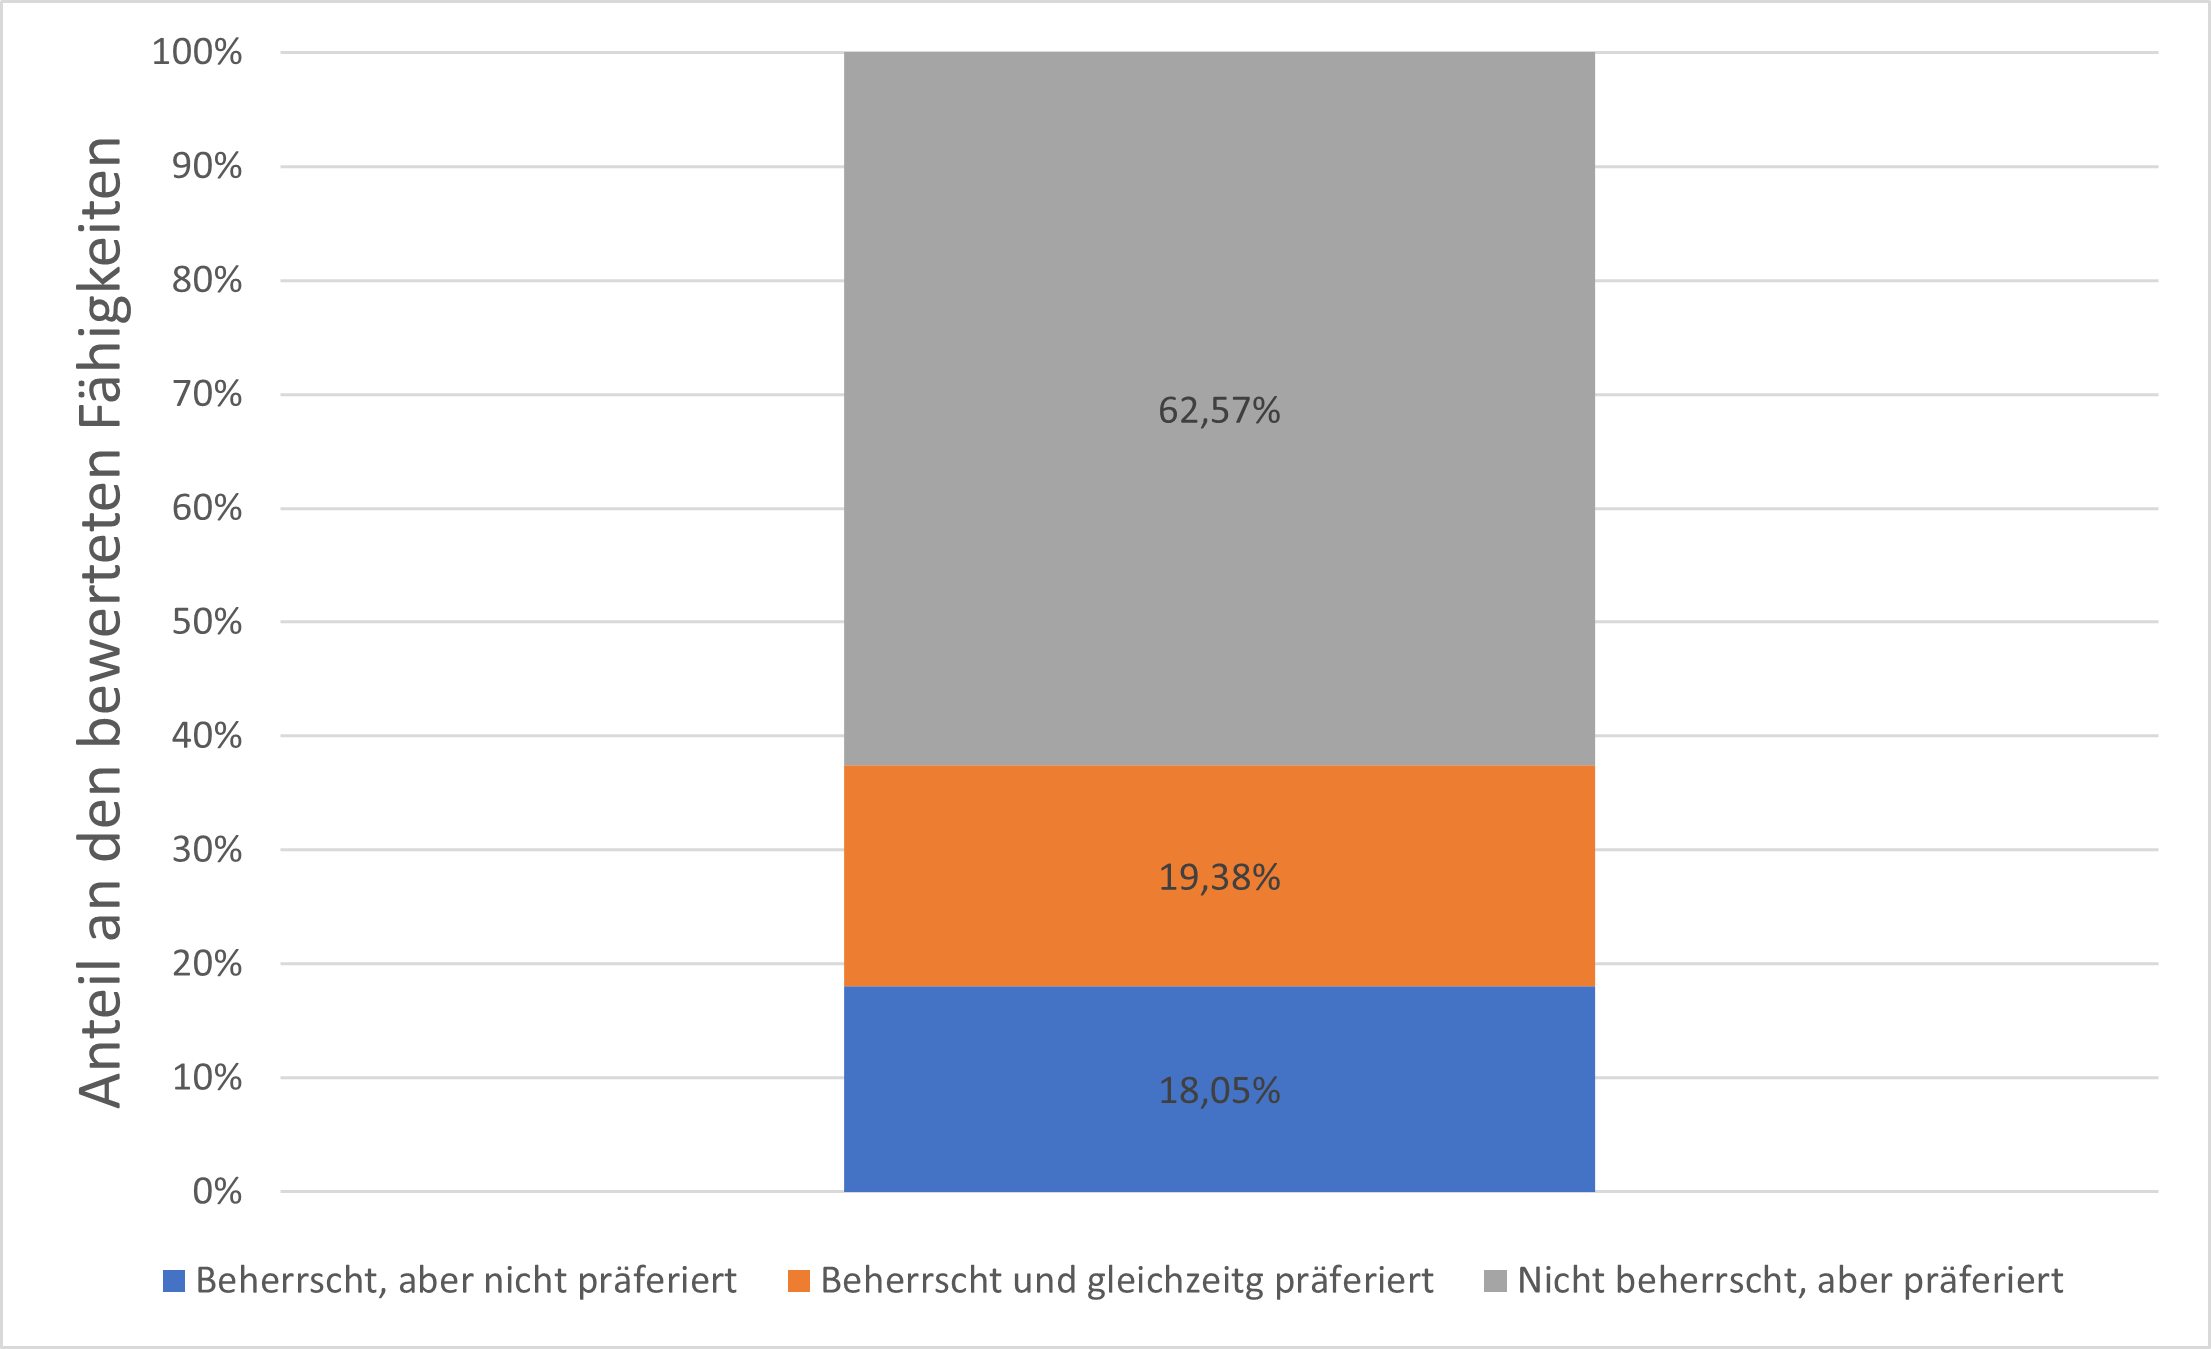
\includegraphics[width=1\textwidth]{gfx/auswertung-anteil-an-faehigkeiten.png}
	\caption{Anteil beherrschter und präferierter Fähigkeiten bei einem durchschnittlichen Mitarbeiter}
	\label{fig:ergebnisse:analyse:abb3}
\end{figure}

In Abbildung \ref{fig:ergebnisse:analyse:abb3} ist zu erkennen, dass ein durchschnittlicher Angestellter etwa 28 bzw. ca. 37.4 Prozent seiner insgesamt beurteilten Kompetenzen gleichzeitig beherrscht (orangene und blaue Farbe). Von diesen Fähigkeiten präferiert er jedoch nur ca. 14.5, also knapp über die Hälfte (orangene Farbe). Demgegenüber stehen ca. 46.7 bzw. etwa 62.6 Prozent an Fähigkeiten, welche der Angestellte zwar präferiert, aber noch nicht beherrscht (graue Farbe).

Im Rahmen der vorliegenden Master-Thesis wurden fünf beispielhafte Projektpositionen definiert und in Kapitel \ref{ch:methodik:evaluation} vorgestellt. Abbildung \ref{fig:ergebnisse:analyse:abb5} zeigt für jede dieser Projektpositionen, wie viele der befragten Mitarbeiter im Durchschnitt die gesuchten Fähigkeiten beherrschen bzw. präferieren.

\begin{figure}[h]
	\centering
	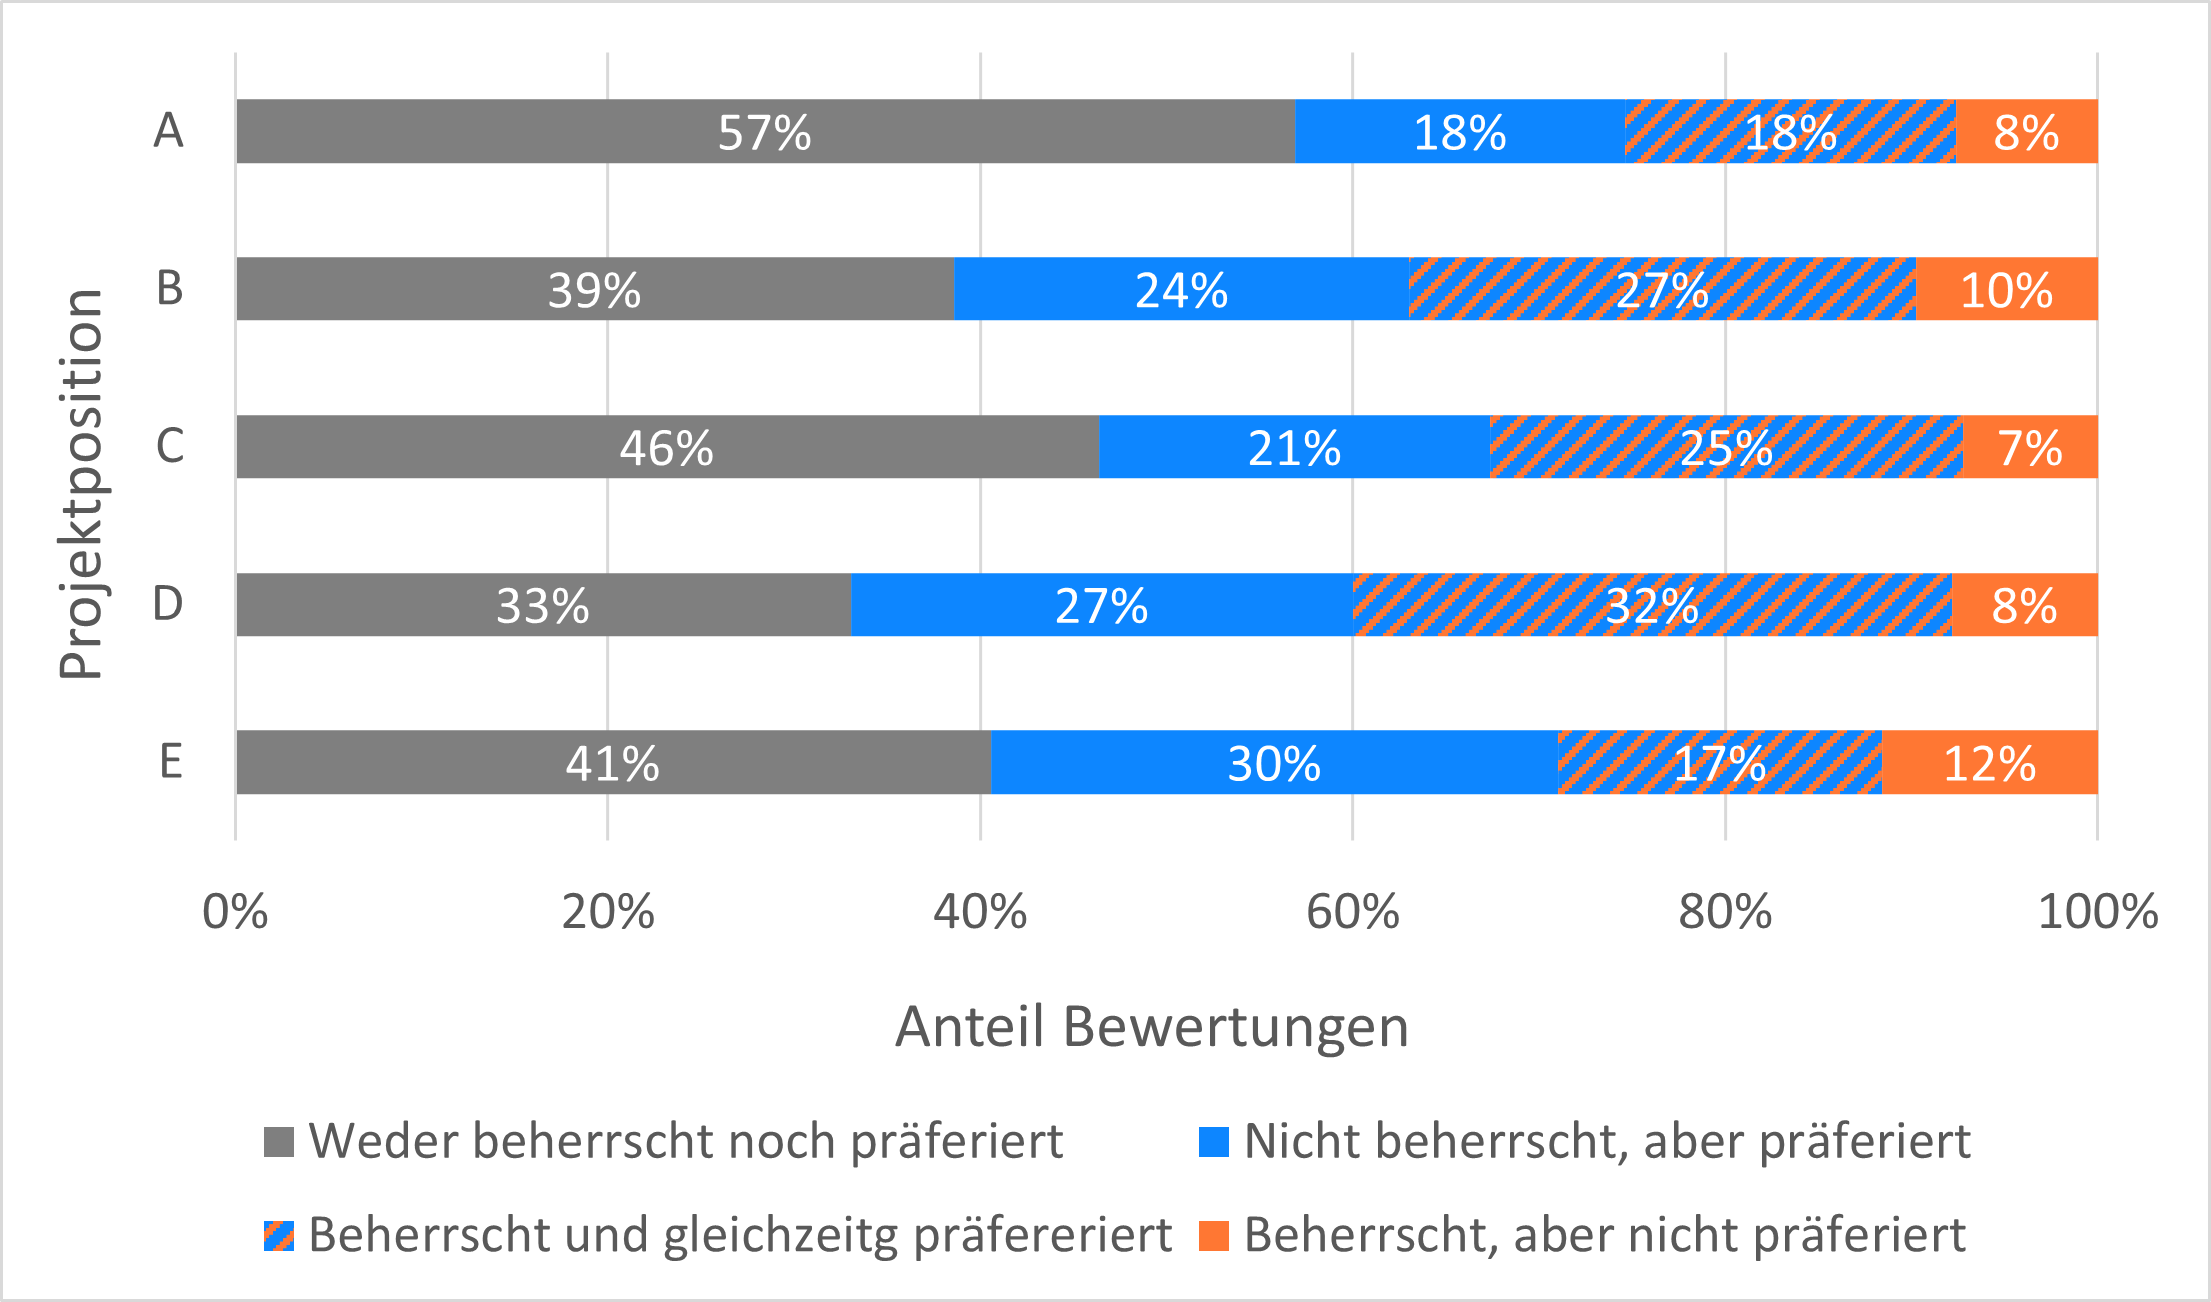
\includegraphics[width=0.85\textwidth]{gfx/anteil-bewertungen-je-projektposition.png}
	\caption{Anteil an Mitarbeitern, welche die in den Beispielprojektpositionen gesuchten Fähigkeiten beherrschen und/oder präferieren}
	\label{fig:ergebnisse:analyse:abb5}
\end{figure}

In Abbildung \ref{fig:ergebnisse:analyse:abb5} ist zu erkennen, dass durchschnittlich 33 Prozent aller Mitarbeiter bereits über die für die Projektpositionen benötigten Fähigkeiten verfügen. Dementsprechend beherrschen 67 Prozent aller Mitarbeiter die durchschnittlich gesuchte Kompetenz noch nicht. Es ist ebenfalls du beobachten, dass 60 Prozent aller Angestellten, welche die durchschnittlich gesuchte Kompetenz beherrschen, diese gleichzeitig präferieren. Auch ist zu erkennen, dass die Anteile an Mitarbeitern, welche die durchschnittlich gesuchte Fähigkeit beherrschen und gleichzeitig präferieren und Angestellten, welche die im Durchschnitt benötigte Kompetenz noch nicht beherrschen und dennoch präferieren mit je 24 Prozent gleich groß sind.

Außerdem ist in den vorliegenden Daten des Intranets zu beobachten, dass vier bzw. 17.4 Prozent der Mitarbeiter keine einzige Fähigkeit bewertet haben. Diese Angestellten sind seit Einführung des Kompetenz-Bewertungssystems durchgehend in einem Projekt tätig und daher von ihrer Führungskraft noch nicht zur Pflege ihrer Fähigkeiten aufgefordert worden. Bei der Umfrage gab es dagegen keinen Mitarbeiter, welcher keine einzige Fähigkeit als Präferenz ausgewählte.

\section{Ergebnisse der Fallstudie}
\label{ch:ergebnisse:fallstudie}

\subsection{Erwartete Zufriedenheit der Projektmitarbeiter}
\label{ch:ergebnisse:fallstudie:umfrageMitarbeiter}
In der in Kapitel \ref{ch:methodik:evaluation} vorgestellten Umfrage wurde erhoben, welche Zufriedenheit die Mitarbeiter der EXXETA AG mit Tätigkeiten auf den Projektpositionen aus Abbildung \ref{fig:methodik:evaluation:abb2} prognostizieren. Die Ergebnisse sind in Abbildung \ref{fig:ergebnisse:fallstudie:abb1} dargestellt.

\begin{figure}[h]
	\centering
	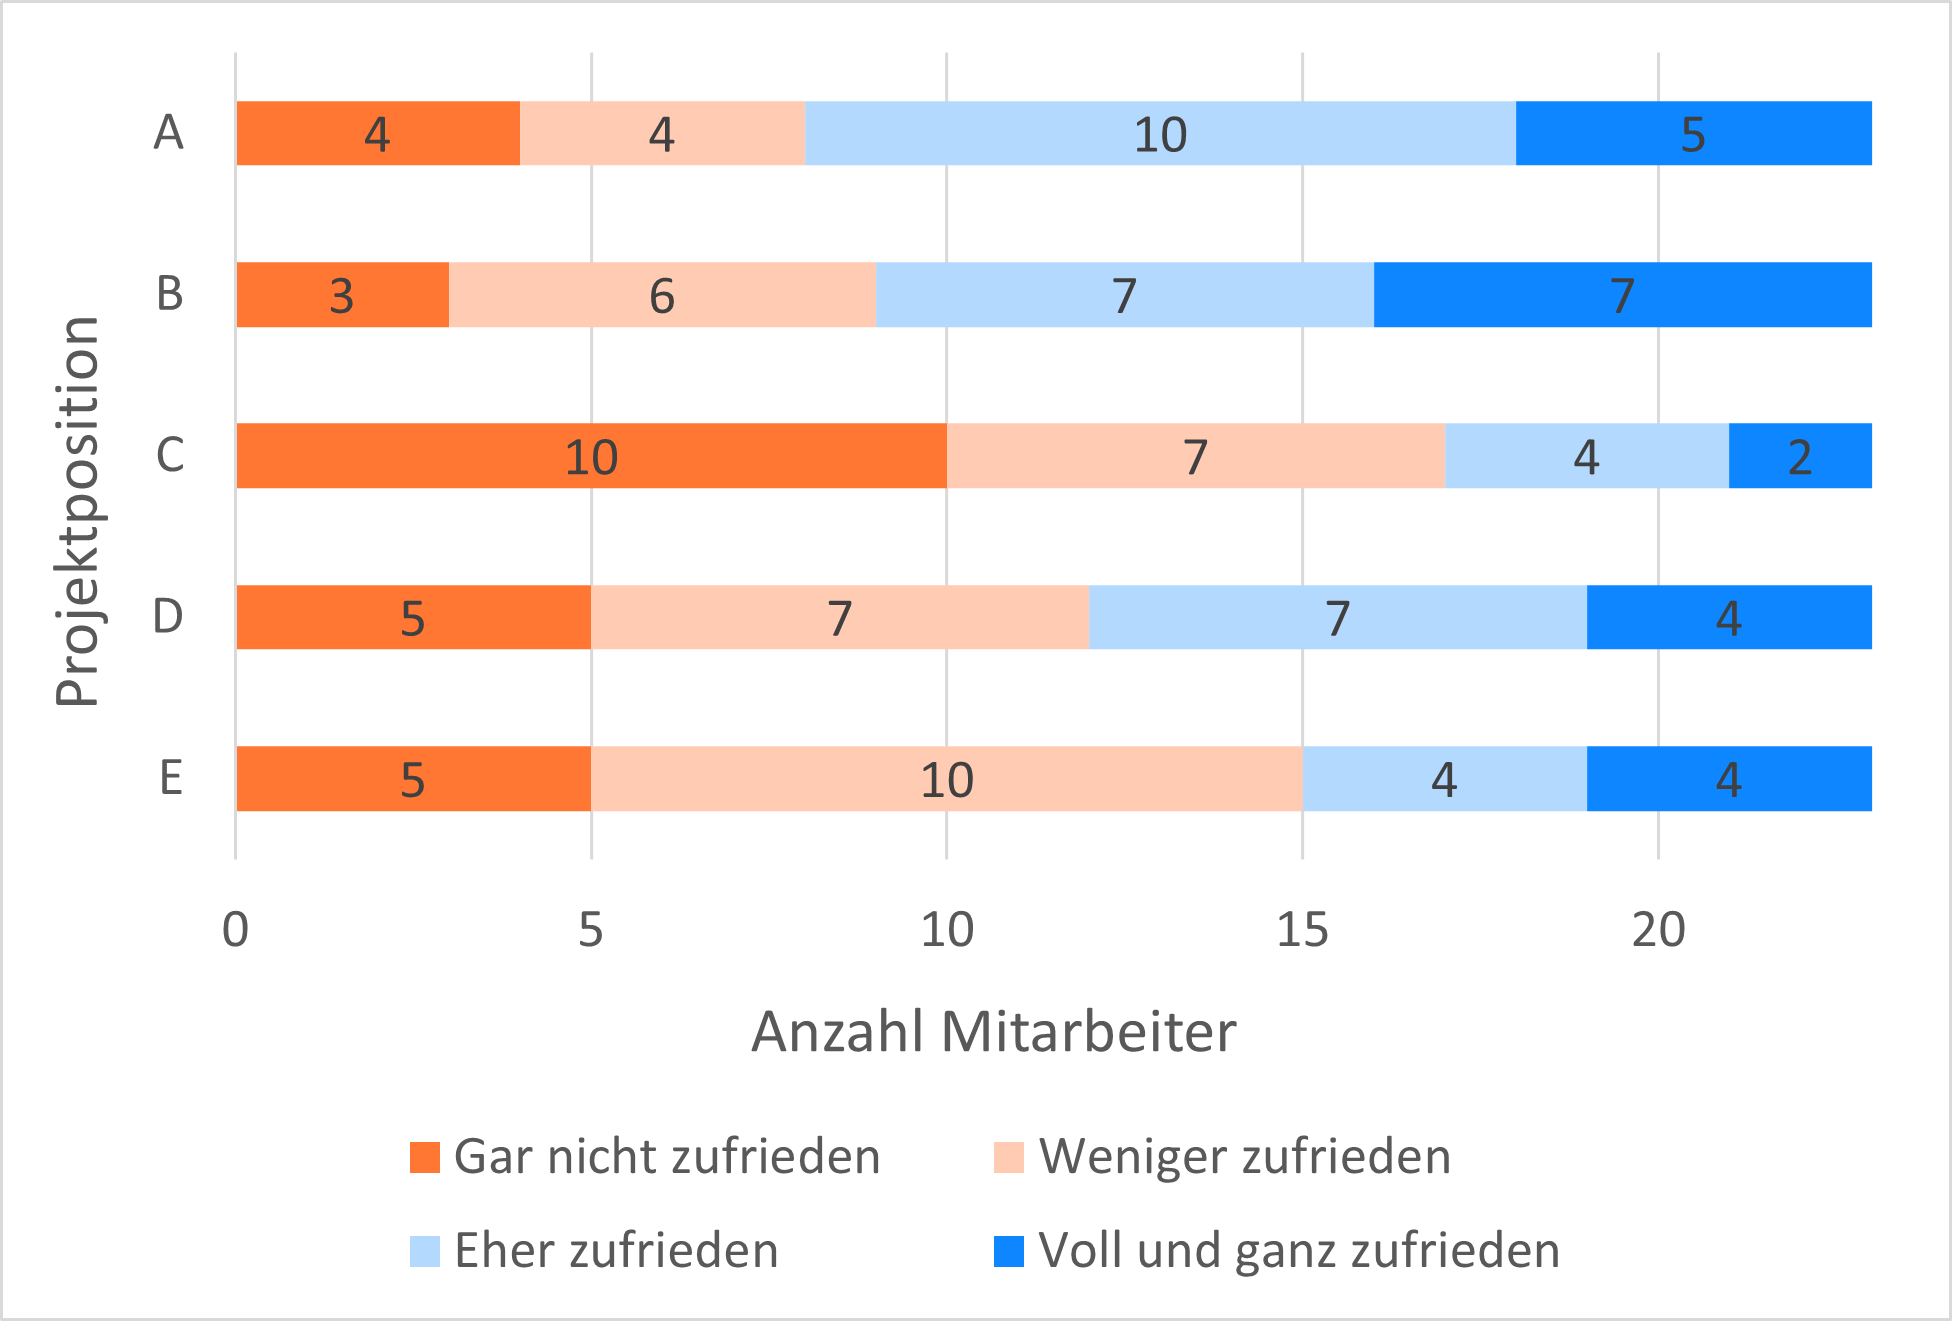
\includegraphics[width=1\textwidth]{gfx/mitarbeiter-zufriedenheit-umfrage.png}
	\caption{Anzahl an Mitarbeitern, welche zufrieden bzw. unzufrieden mit der Tätigkeit auf den jeweiligen Beispielprojektpositionen wären}
	\label{fig:ergebnisse:fallstudie:abb1}
\end{figure}

In Abbildung \ref{fig:ergebnisse:fallstudie:abb1} ist zu erkennen, dass die Mitarbeiter überwiegend eine hohe Zufriedenheit mit den Projektpositionen A und B prognostizieren. Mit einer Tätigkeit auf den Projektpositionen C und E zeigen sich die Angestellten eher unzufrieden. Projektposition D stehen die Mitarbeiter gespalten gegenüber, sodass etwa die Hälfte der Befragten zufrieden und die andere Hälfte unzufrieden mit dieser Tätigkeit wäre.

Abbildung \ref{fig:ergebnisse:analyse:abb7} zeigt, für wie viele der 23 befragten Mitarbeiter der bilaterale Empfehlungsansatz gegenüber dem unilateralen Vorgehen für eine höhere Zufriedenheit seitens der Mitarbeiter sorgte. Wie in Kapitel \ref{ch:methodik:evaluation} beschrieben, entsteht eine höhere Zufriedenheit mit den Projekttätigkeiten, wenn das bilaterale System die Angestellten bei einer prognostizierten Zufriedenheit höher und bei einer erwarteten Unzufriedenheit niedriger positioniert als die unilaterale Anwendung.

\begin{figure}[h]
	\centering
	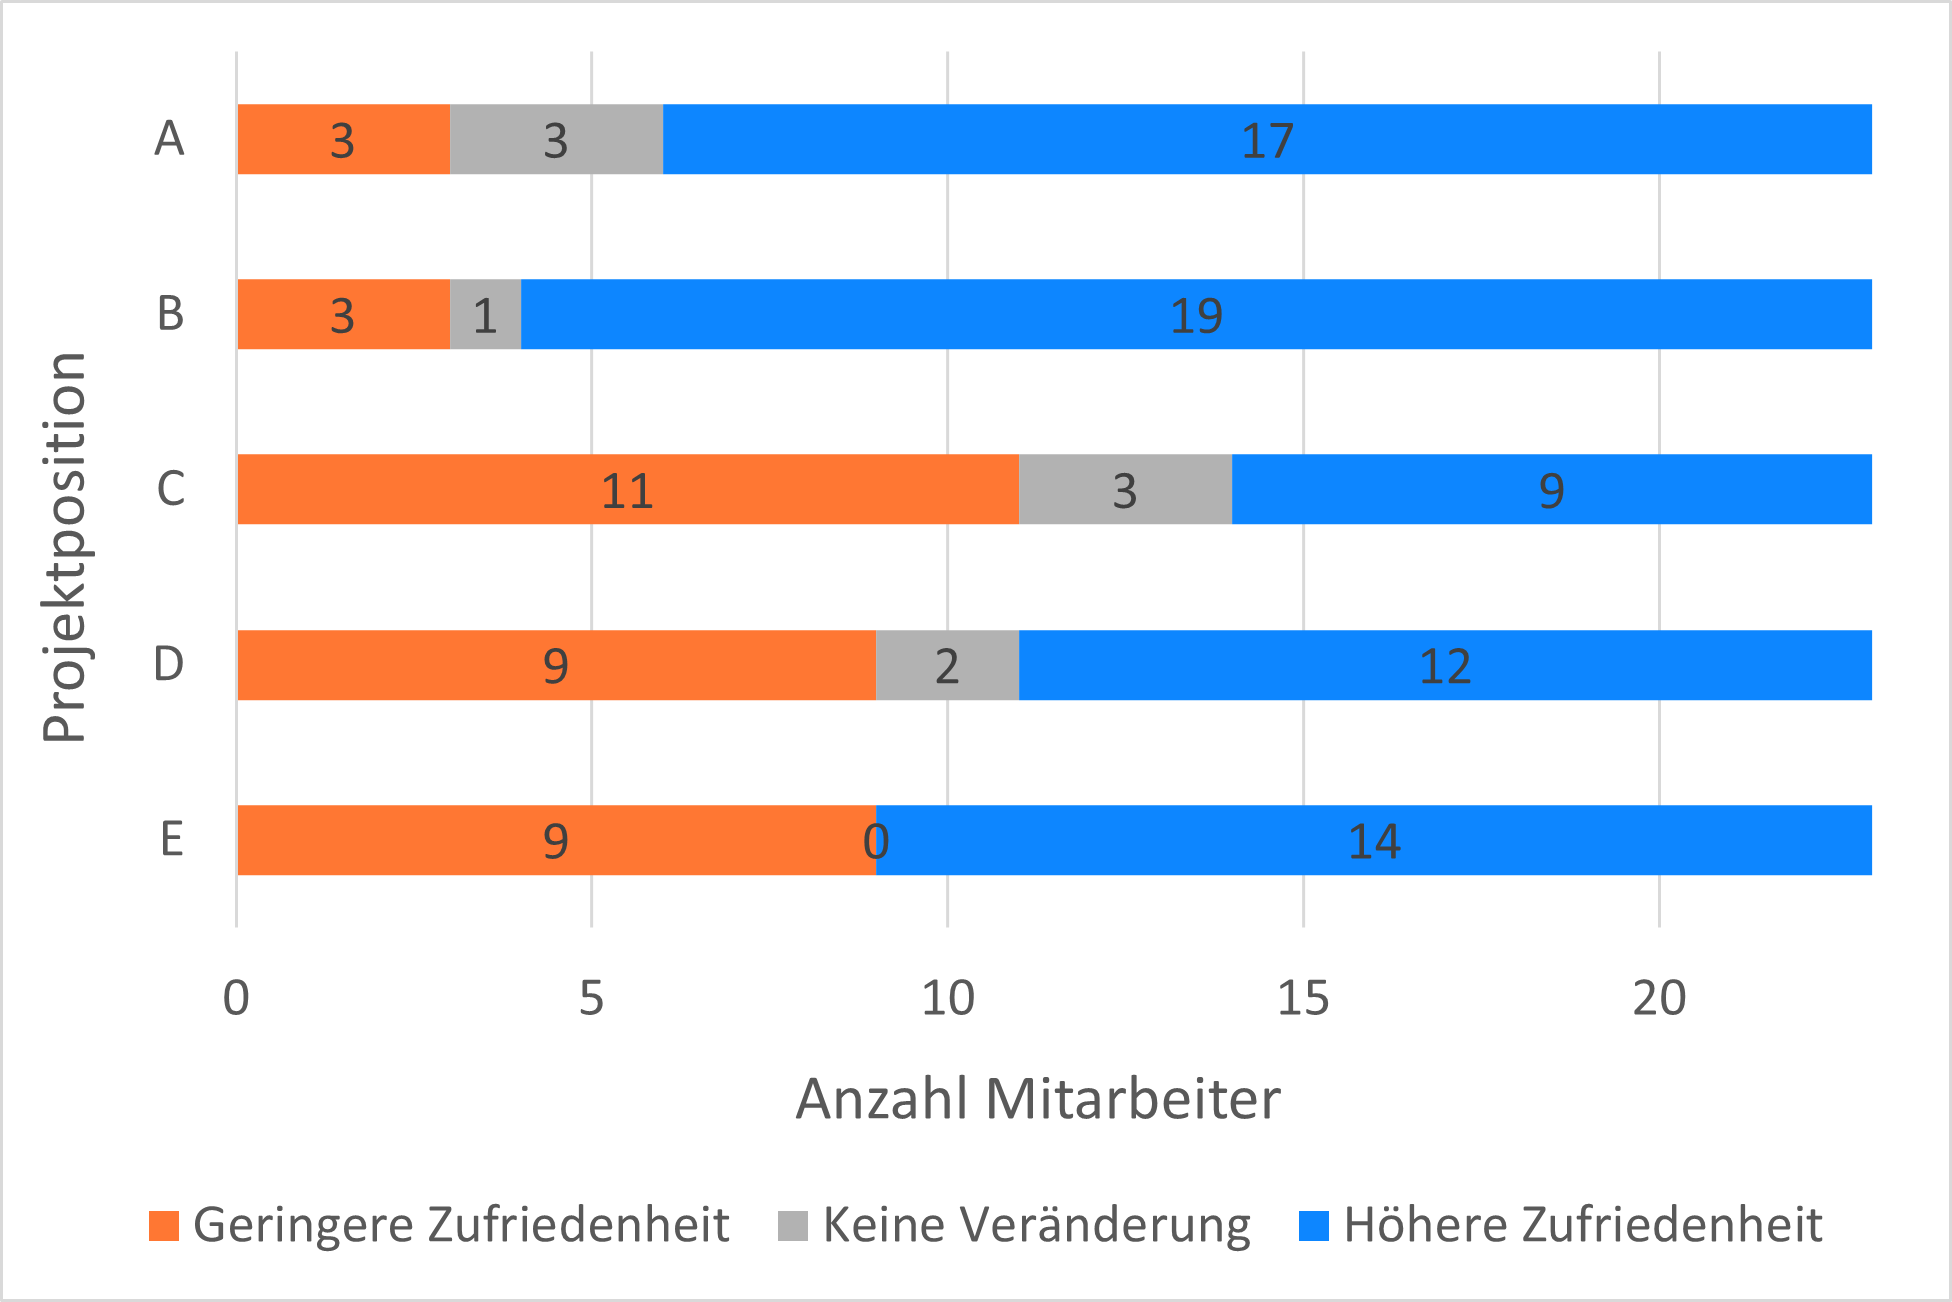
\includegraphics[width=1\textwidth]{gfx/zufriedenheit-projekte.png}	
	\caption{Ergebnisse des bilateralen Empfehlungsansatzes im Vergleich zum unilateralen Vorgehen hinsichtlich der Mitarbeiterzufriedenheit}
	\label{fig:ergebnisse:analyse:abb7}
\end{figure}

In Abbildung \ref{fig:ergebnisse:analyse:abb7} ist zu erkennen, dass der bilaterale Empfehlungsansatz einen Großteil der Angestellten für die Projektpositionen A und B zugunsten einer höheren Zufriedenheit positionierte. Bei den Projektpositionen D und E sind erreiche das bilaterale Vorschlagsverfahren für knapp über die Hälfte der Mitarbeiter eine höhere Zufriedenheit. Bei Projektposition C konnte dagegen der unilaterale Empfehlungsansatz für den Großteil der Angestellten eine höhere Zufriedenheit erzielen.

\subsection{Prognostizierte Arbeitsleistung der Projektmanager}
\label{ch:ergebnisse:fallstudie:arbeitsleistung}
An der Umfrage unter den Projektmanagern haben N=sechs Personen teilgenommen. Fünf der Teilnehmer sind im Bereich \acl{JES} tätig. Eine Person stammt aus einer anderen Abteilung, welche ähnliche Technologien bei der Projekttätigkeit einsetzt.

Abbildung \ref{fig:ergebnisse:fallstudie:arbeitsleistung:abb1} zeigt, von den Mitarbeitern der Listen welches Empfehlungsansatzes die Projektmanager eine höhere Arbeitsleistung erwarten.

\begin{figure}[h]
	\centering
	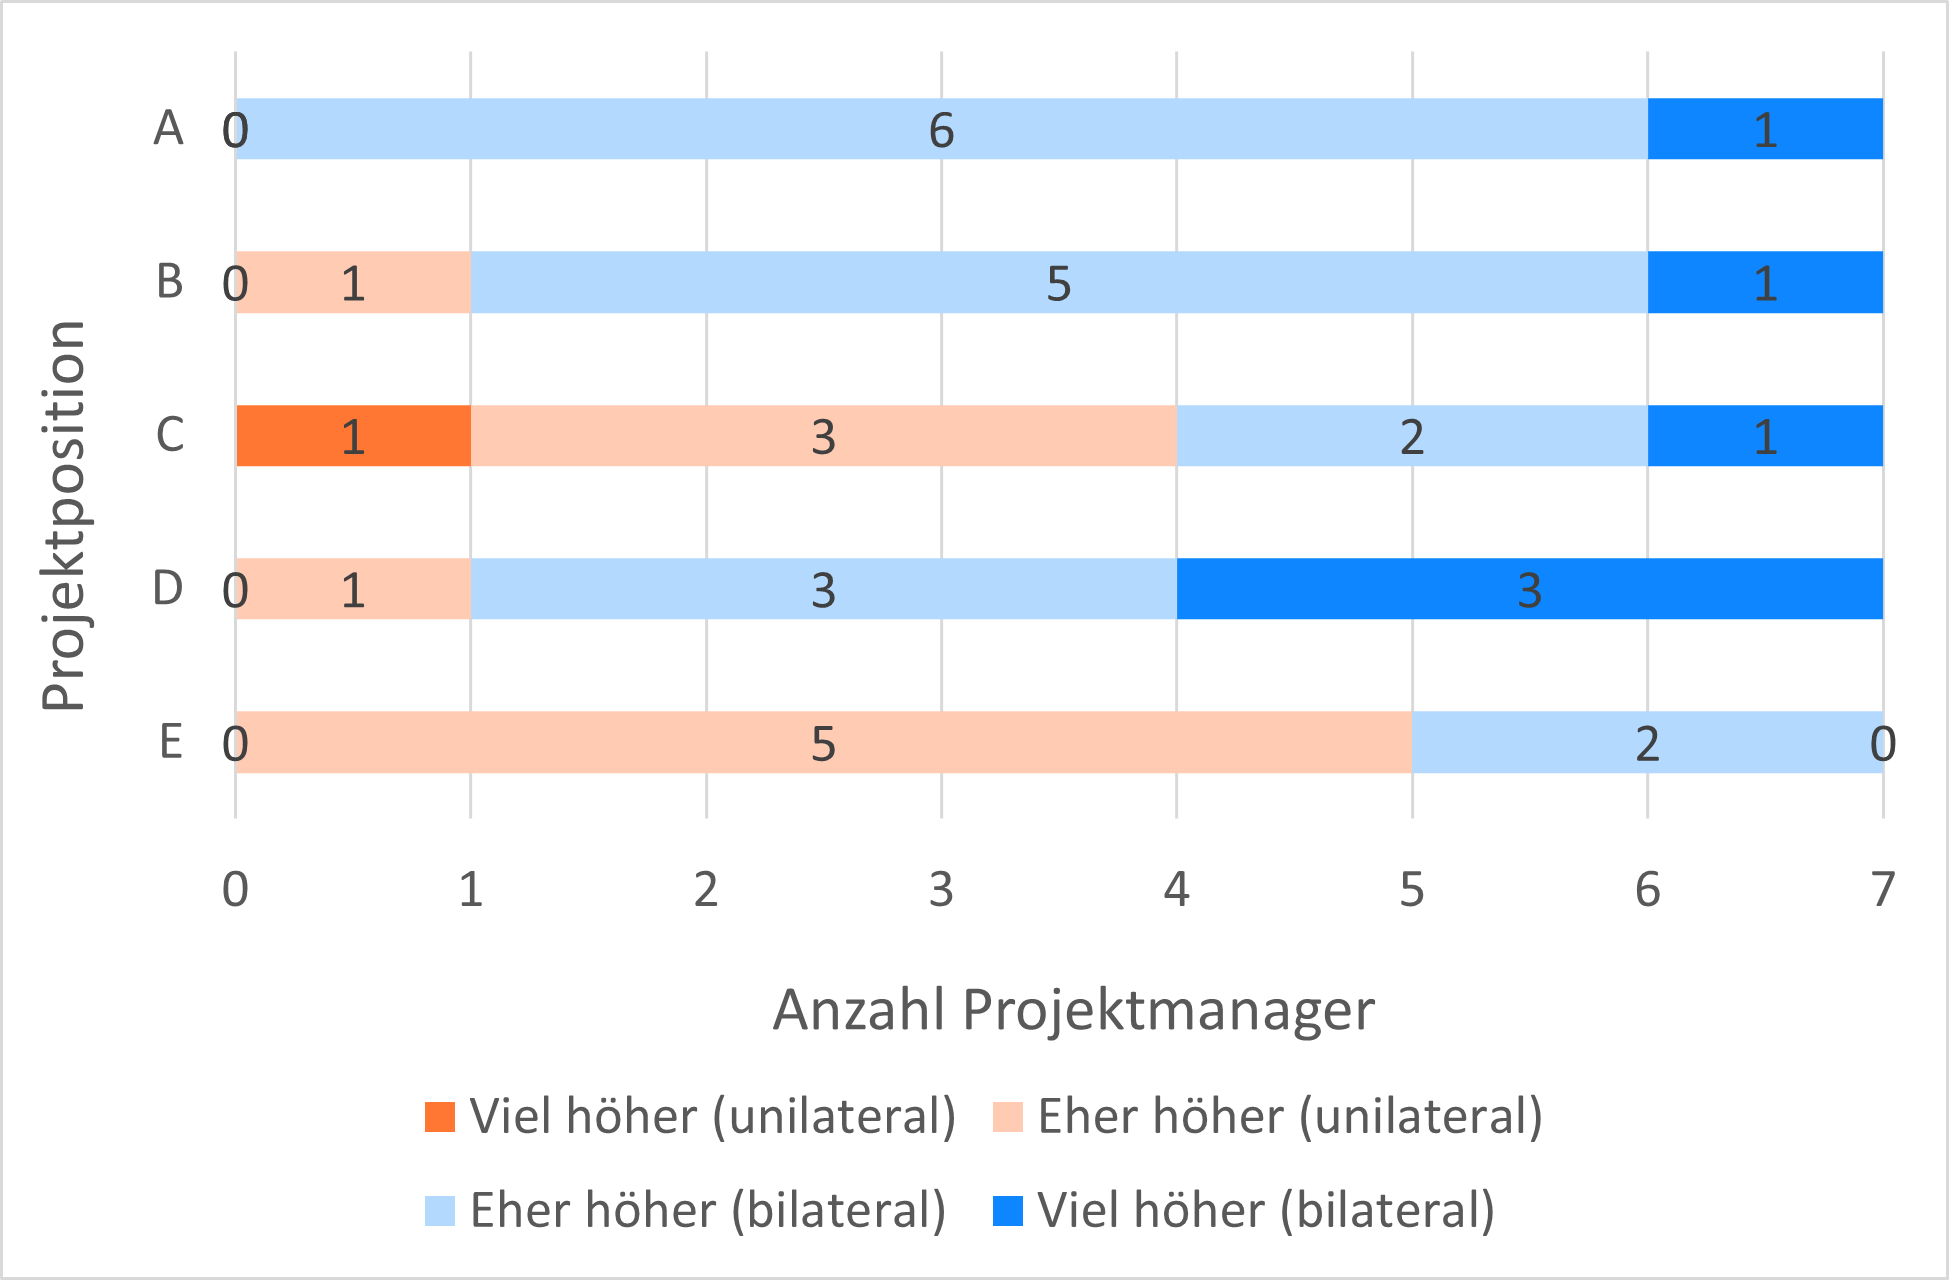
\includegraphics[width=1\textwidth]{gfx/ergebnisse-projektmanager-arbeitsleistung.png}	
	\caption{Ergebnisse der Umfrage unter den Projektmanager hinsichtlich der erwarteten Arbeitsleistung der Mitarbeiter}
	\label{fig:ergebnisse:fallstudie:arbeitsleistung:abb1}
\end{figure}

An den Ergebnissen aus Abbildung \ref{fig:ergebnisse:fallstudie:arbeitsleistung:abb1} ist zu erkennen, dass die Projektmanager bei vier der fünf Projektpositionen von den vorgeschlagenen Mitarbeitern des bilateralen Empfehlungsansatzes eine höhere Arbeitsleistung erwarten. Für Projektposition A ist zu beobachten, dass kein einziger Projektmanager eine höhere Leistung von den unilateralen Empfehlungen erwartet. Auffällig ist außerdem, dass die Hälfte der Teilnehmer von den Vorschlägen des bilateralen Empfehlungssystems für Projektposition D eine viel höhere Arbeitsleistung erwartet.

Einzig bei den Vorschläge für Projektposition C in Abbildung \ref{fig:ergebnisse:fallstudie:arbeitsleistung:abb1} sind keine Unterschiede zwischen der erwarteten Arbeitsleistung des uni- und des bilateralen Empfehlungssystems erkennbar.



\subsection{Einschätzungen hinsichtlich möglicher Unterforderung}
\label{ch:ergebnisse:fallstudie:kurven}
\shorthandon{"}
